
\chapter{Organisation of the work}

\section{Calendar}


\begin{tabular*}{1\textwidth}{@{\extracolsep{\fill}} |c|*{14}{c|}}
\hline
  Tasks/weeks & 1 &2 &3&4&5&6&7&8&9&10&11&12&13&14\\
\hline
State of the art&-&-&&&&&&&&X&&&&\\
\hline
Create a plugin&&&-&&&&&&&X&&&&\\
\hline
Visualize the simulation&&&&-&-&-&-&-&&X&&&&\\
\hline
Unit tests&&&&&&&&-&&X&&&&\\
\hline
Integration tests&&&&&&&&&-&X&&&&\\
\hline
Try an other simulator&&&&&&&&&&X&-&-&&\\
\hline
Redaction&&-&-&-&-&-&-&-&-&X&-&-&-&\\
\hline
Oral&&&&&&-&&&&X&&&&-\\
\hline
\end{tabular*}

~\\

During the week 10, the University was closed, that is why it is a trivialized week.

\section{Tools use for the project}

The Framaboard application:

\begin{figure}[h]
  \centering
  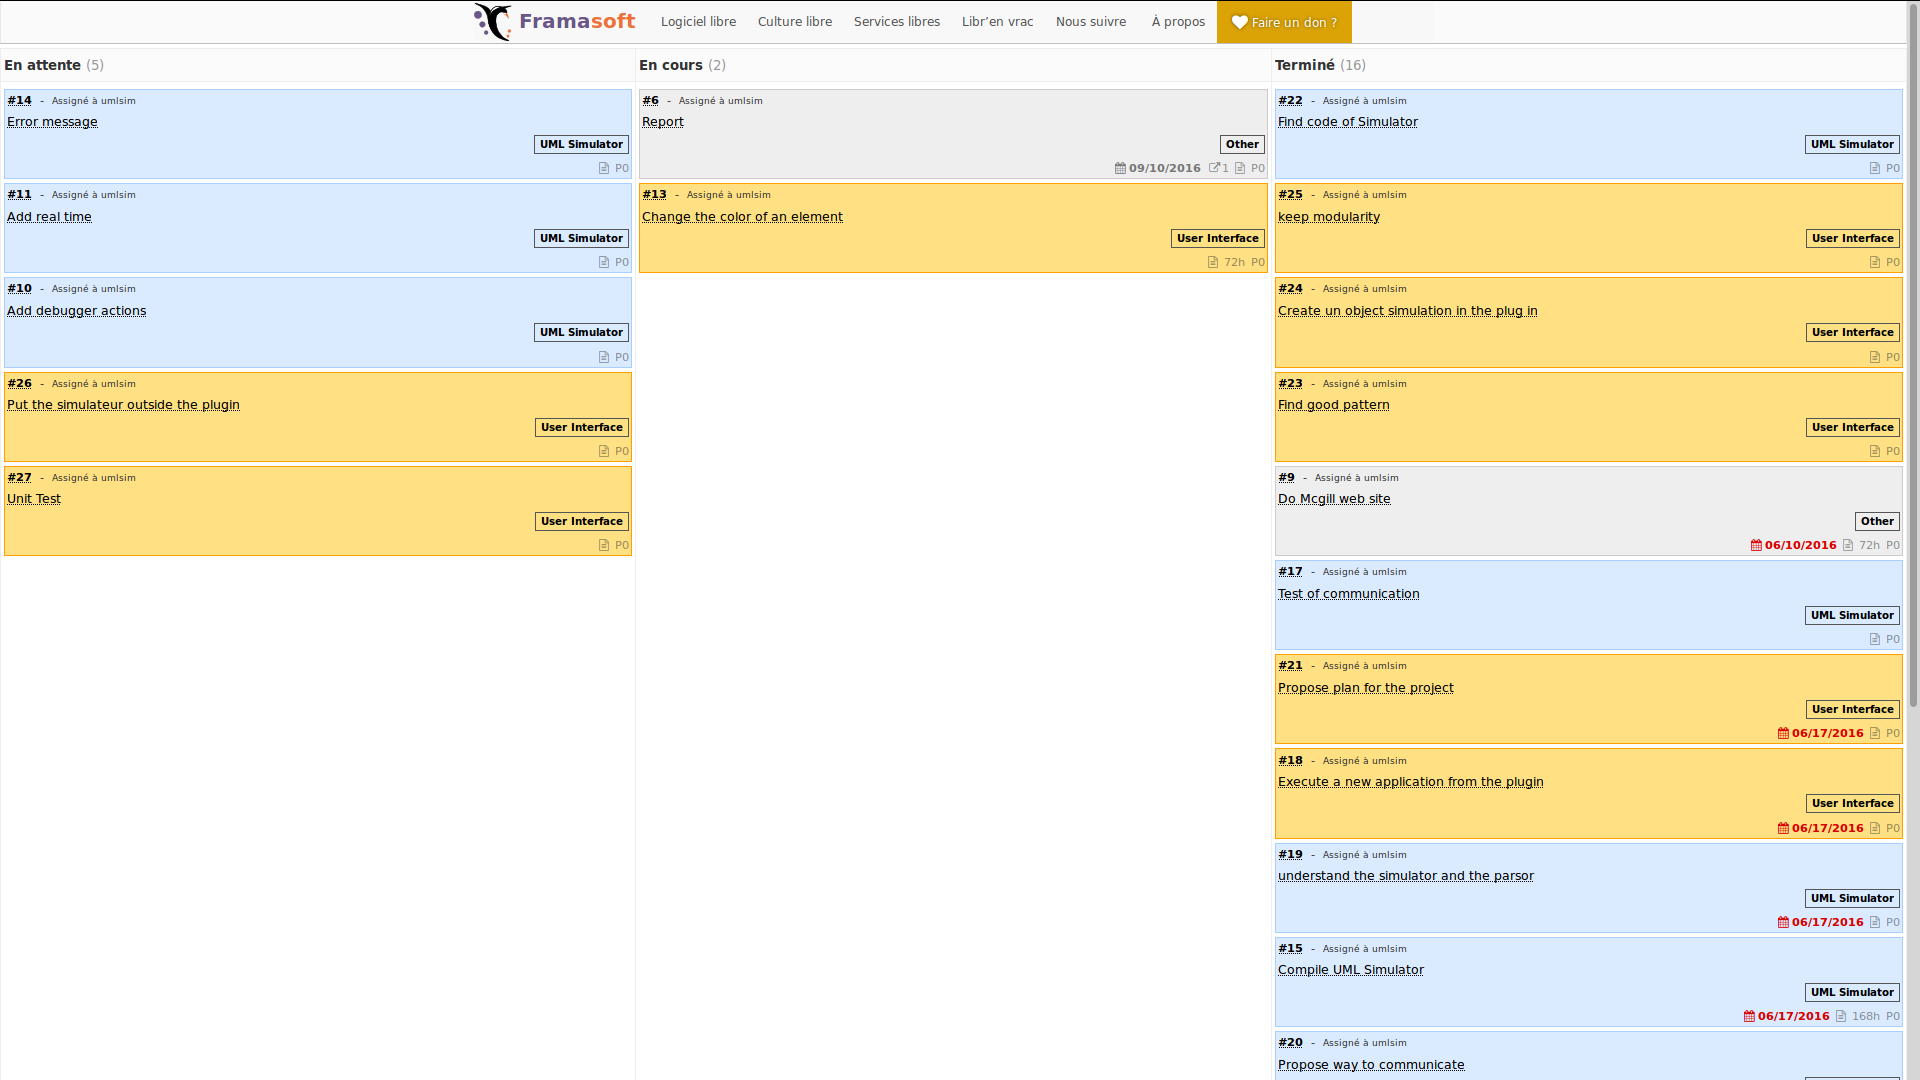
\includegraphics[width=\textwidth]{framaboard}
  \caption{Screen shot of the framaboard}
  \label{fig:framaboard}
\end{figure}


The web site of MSDL researcher:

\begin{figure}[h]
  \centering
  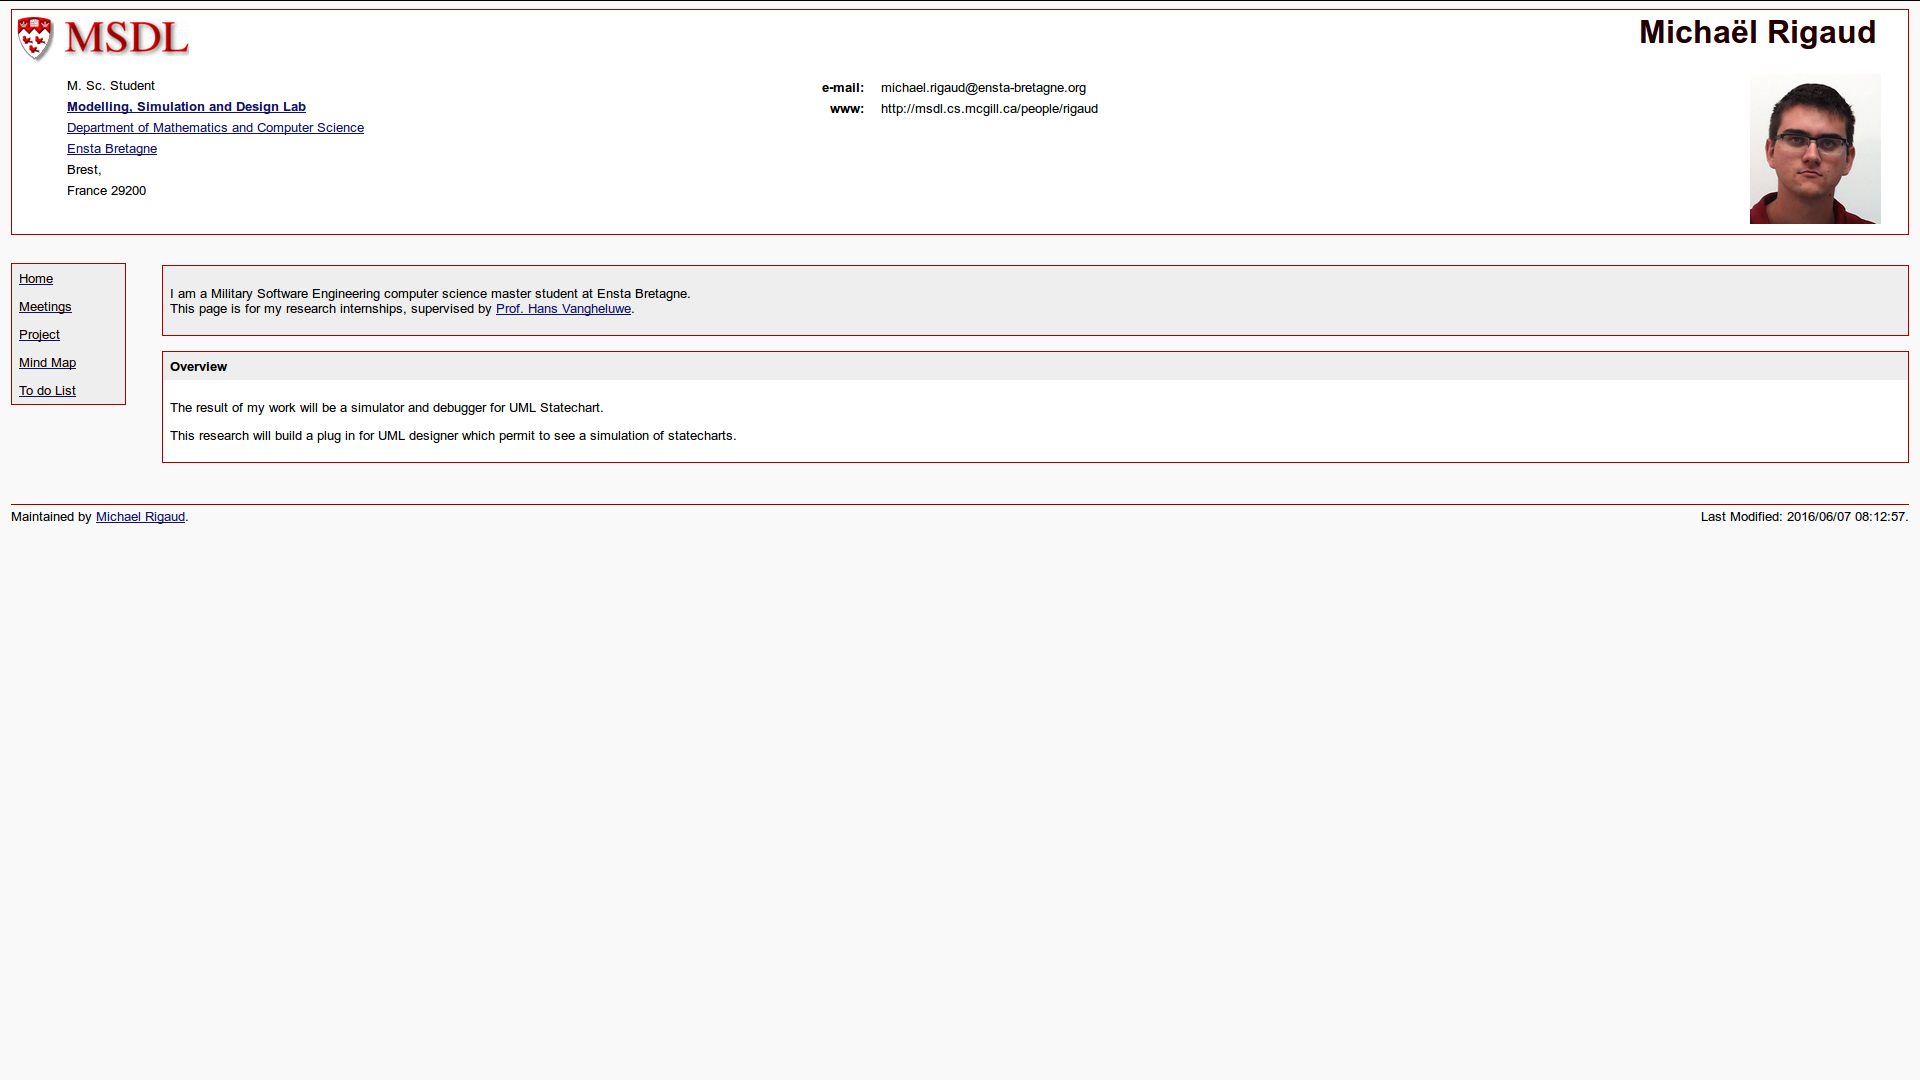
\includegraphics[width=\textwidth]{msdl}
  \caption{MSDL web site}
  \label{fig:msdl}
\end{figure}


The MSDL git repository

\begin{figure}[h]
  \centering
  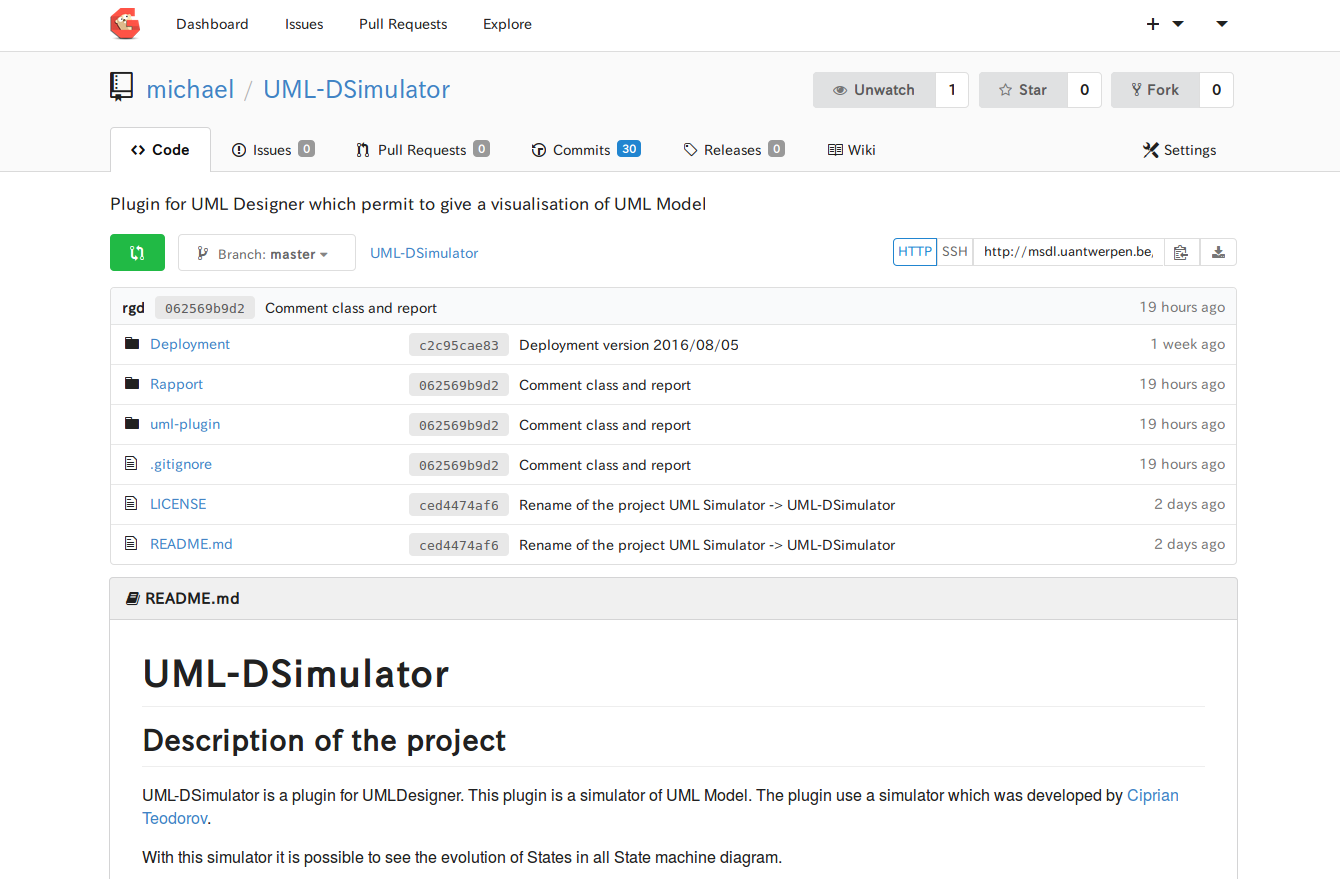
\includegraphics[width=\textwidth]{git.png}
  \caption{git repository}
  \label{fig:git}
\end{figure}



%%% Local Variables:
%%% mode: latex
%%% TeX-master: "../rapport_de_base"
%%% End:
